% !TEX root = ../em1_pset_v2.tex
\Opensolutionfile{solution_file}[solutions/sols_140]
% в квадратных скобках фактическое имя файла

\chapter{Классификационные деревья и алгоритм случайного леса}


\begin{problem}
Для случайных величин  $X$ и $Y$ найдите индекс Джини и энтропию.


\begin{tabular}{ccc}
\toprule
$X$ & $0$ & $1$ \\
$\P()$ & $0.2$ & $0.8$ \\
\bottomrule
\end{tabular},
\begin{tabular}{cccc}
\toprule
$Y$ & $0$ & $1$ & $5$ \\
$\P()$ & $0.2$ & $0.3$ & $0.5$ \\
\bottomrule
\end{tabular}


\begin{sol}
$I_X = 1 - 0.2^2 - 0.8^2 = 0.32$, $H(X) = -(0.2 \ln 0.2 + 0.8 \ln 0.8) \approx 0.5$

$I_Y = 1 - 0.2^2 - 0.3^2 - 0.5^2 = 0.62$, $H(Y) = -(0.2 \ln 0.2 + 0.3 \ln 0.3 + 0.5 \ln 0.5) \approx 1.03$

\end{sol}
\end{problem}


\begin{problem}
Случайная величина $X$ принимает значение $1$ с вероятностью $p$ и значение $0$ с вероятностью $1-p$.
\begin{enumerate}
\item Постройте график зависимости индекса Джини и энтропии от $p$.
\item Являются ли функции монотонными? выпуклыми?
\item При каком $p$ энтропия и индекс Джини будут максимальны?
\end{enumerate}


\begin{sol}
$I = 2p(1-p)$, энтропия и индекс Джини максимальны при $p=0.5$.
\end{sol}
\end{problem}



\begin{problem}
Кот Леопольд анкетировал 20 мышей по трём вопросам: $x$ — «Одобряете ли Вы непримиримую к котам позицию Белого и Серого?», $y$ — «Известно ли Вам куда пропала моя любимая кошка Мурка?» и $z$ — «Известны ли Вам настоящие имена Белого и Серого?» Результаты опроса в таблице:

\begin{tabular}{rlll}
  \hline
 & x & y & z \\ 
  \hline
1 & no & no & yes \\ 
  2 & no & yes & yes \\ 
  3 & yes & yes & yes \\ 
  4 & yes & yes & no \\ 
  5 & no & no & no \\ 
  6 & no & yes & yes \\ 
  7 & no & no & yes \\ 
  8 & no & no & no \\ 
  9 & yes & no & yes \\ 
  10 & yes & no & yes \\ 
  11 & no & no & no \\ 
  12 & yes & yes & yes \\ 
  13 & no & yes & yes \\ 
  14 & no & yes & no \\ 
  15 & yes & no & no \\ 
  16 & yes & no & yes \\ 
  17 & no & no & no \\ 
  18 & no & yes & no \\ 
  19 & no & yes & no \\ 
  20 & yes & no & no \\ 
   \hline
\end{tabular}

\begin{minted}[mathescape, numbersep=5pt, frame=lines, framesep=2mm]{r}
set.seed(1975)
x <- sample(c("yes", "no"), size = 20, rep = TRUE)
y <- sample(c("yes", "no"), size = 20, rep = TRUE)
z <- sample(c("yes", "no"), size = 20, rep = TRUE)
xtable(data_frame(x, y, z))
\end{minted}



\begin{enumerate}
\item Какой фактор нужно использовать при прогнозировании $y$, чтобы минимизировать энтропию?
\item Какой фактор нужно использовать при прогнозировании $y$, чтобы минимизировать индекс Джини?
\end{enumerate}


\begin{sol}
\end{sol}
\end{problem}





\begin{problem}
Постройте регрессионное дерево для набора данных:

\begin{tabular}{cc}
\toprule
$y_i$ & $x_i$ \\
\midrule
$5$ & $0$ \\
$6$ & $1$ \\
$4$ & $2$ \\
$100$ & $3$ \\
\bottomrule
\end{tabular}

Критерий деления узла на два — минимизация $RSS$. Дерево строится до трёх терминальных узлов.


\begin{sol}
Первое разбиение по порогу $x_i < 2.5$, второе — по $x_i < 1.5$.
\end{sol}
\end{problem}

\begin{problem}
Постройте регрессионное дерево для набора данных:

\begin{tabular}{cc}
\toprule
$y_i$ & $x_i$ \\
\midrule
$100$ & $1$ \\
$102$ & $2$ \\
$103$ & $3$ \\
$50$ & $4$ \\
$55$ & $5$ \\
$61$ & $6$ \\
$70$ & $7$ \\
\bottomrule
\end{tabular}

Критерий деления узла на два — минимизация $RSS$. Узлы делятся до тех пор, пока в узле остаётся больше двух наблюдений.
\begin{sol}
Первое разбинение по порогу $x_i < 3.5$. Левый лист разбивается по порогу $x_i < 5.5$, правый — по порогу $x_i < 1.5$.
\end{sol}
\end{problem}




\begin{problem}
Дон-Жуан предпочитает брюнеток. Перед Новым Годом он посчитал, что в записной книжке у него 20 блондинок, 40 брюнеток, две рыжих и восемь шатенок. С Нового Года Дон-Жуан решил перенести все сведения в две записные книжки, в одну — брюнеток, во вторую — остальных.

Как изменились индекс Джини и энтропия в результате такого разбиения?
\begin{sol}
Было: $I = 1 - \left(\frac{20}{70}\right)^2 - \left(\frac{40}{70}\right)^2- \left(\frac{2}{70}\right)^2- \left(\frac{8}{70}\right)^2 = \frac{708}{1225} \approx 0.58$,

$H =-\left( \frac{20}{70} \ln \frac{20}{70} +  \frac{40}{70} \ln \frac{40}{70} +  \frac{2}{70} \ln \frac{2}{70} +  \frac{8}{70} \ln \frac{8}{70}  \right) \approx 1.03$.

Стало: $I_L = 0$, $I_R = 1 - \left(\frac{20}{30}\right)^2 - \left(\frac{2}{30}\right)^2 - \left(\frac{8}{30}\right)^2 = 0.48$, $I = \frac{40}{70}\cdot 0 + \frac{30}{70} \cdot 0.48 \approx 0.21$,

$H_L = 0$, $H_R = -\left(\frac{20}{30} \ln \frac{20}{30} + \frac{2}{30} \ln \frac{2}{30} + \frac{8}{30} \ln \frac{8}{30} \right) \approx 0.8$, $H =  \frac{40}{70}\cdot 0 + \frac{30}{70} \cdot 0.8 \approx 0.34$.

\end{sol}
\end{problem}



\begin{problem}
Машка пять дней подряд гадала на ромашке, а затем выкладывала очередную фотку «Машка с ромашкой» в инстаграмчик. Результат гадания — переменная $y_i$, количество лайков у фотки — переменная $x_i$. Постройте классификационное дерево.

\begin{tabular}{cc}
$y_i$ & $x_i$ \\
\hline
плюнет & $10$ \\
поцелует & $11$ \\
поцелует & $12$ \\
к сердцу прижмёт & $13$ \\
к сердцу прижмёт & $14$ \\
\end{tabular}

Дерево строится до идеальной классификации. Критерий деления узла на два — максимальное падение индекса Джини.


\begin{sol}
Первое разбиение по порогу $x_i < 12.5$, второе — по порогу $x_i < 10.5$.
\end{sol}
\end{problem}




\begin{problem}
У Винни-Пуха есть 100 песенок (кричалок, вопелок, пыхтелок и сопелок). 
Каждый день он выбирает и поёт одну из них равновероятно наугад. 
Одну и ту же песенку он может петь несколько раз. 
Сколько в среднем песенок оказываются неспетыми за 100 дней?


\begin{sol}
$100\cdot \left(\frac{99}{100} \right)^{100}\approx 100/e \approx 37$
\end{sol}
\end{problem}


\begin{problem}
По данной диаграмме рассеяния постройте классификационное дерево для зависимой переменной $y$:

\begin{minted}[mathescape, numbersep=5pt, frame=lines, framesep=2mm]{r}
set.seed(42)
df <- tibble(x = runif(400), z = runif(400))
df$y <- factor(ifelse(df$x > 0.25 & df$z > 0.5, "yes", "no"))
qplot(data = df, x = x, y = z, col = y, shape = y) +
    geom_vline(xintercept = 0.25) + geom_hline(yintercept = 0.5)
\end{minted}


\begin{minipage}{0.6\textwidth}
\begin{center}
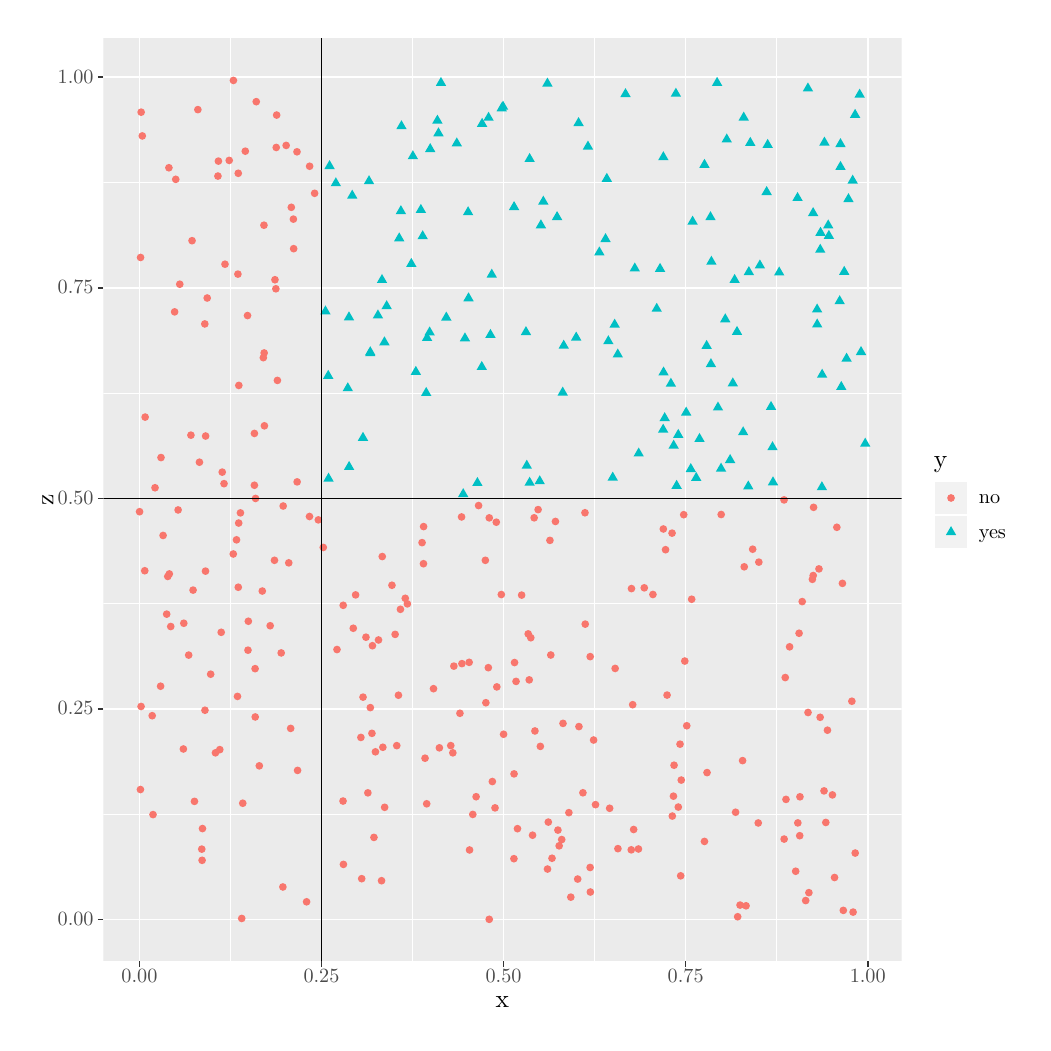
\begin{tikzpicture}[scale = 0.025]
% Created by tikzDevice version 0.12 on 2019-05-28 10:06:31
% !TEX encoding = UTF-8 Unicode
\definecolor{fillColor}{RGB}{255,255,255}
\path[use as bounding box,fill=fillColor,fill opacity=0.00] (0,0) rectangle (505.89,505.89);
\begin{scope}
\path[clip] (  0.00,  0.00) rectangle (505.89,505.89);
\definecolor{drawColor}{RGB}{255,255,255}
\definecolor{fillColor}{RGB}{255,255,255}

\path[draw=drawColor,line width= 0.6pt,line join=round,line cap=round,fill=fillColor] (  0.00,  0.00) rectangle (505.89,505.89);
\end{scope}
\begin{scope}
\path[clip] ( 38.43, 31.51) rectangle (444.01,500.39);
\definecolor{fillColor}{gray}{0.92}

\path[fill=fillColor] ( 38.43, 31.51) rectangle (444.01,500.39);
\definecolor{drawColor}{RGB}{255,255,255}

\path[draw=drawColor,line width= 0.3pt,line join=round] ( 38.43,106.16) --
	(444.01,106.16);

\path[draw=drawColor,line width= 0.3pt,line join=round] ( 38.43,213.20) --
	(444.01,213.20);

\path[draw=drawColor,line width= 0.3pt,line join=round] ( 38.43,320.24) --
	(444.01,320.24);

\path[draw=drawColor,line width= 0.3pt,line join=round] ( 38.43,427.27) --
	(444.01,427.27);

\path[draw=drawColor,line width= 0.3pt,line join=round] (103.04, 31.51) --
	(103.04,500.39);

\path[draw=drawColor,line width= 0.3pt,line join=round] (195.55, 31.51) --
	(195.55,500.39);

\path[draw=drawColor,line width= 0.3pt,line join=round] (288.07, 31.51) --
	(288.07,500.39);

\path[draw=drawColor,line width= 0.3pt,line join=round] (380.59, 31.51) --
	(380.59,500.39);

\path[draw=drawColor,line width= 0.6pt,line join=round] ( 38.43, 52.65) --
	(444.01, 52.65);

\path[draw=drawColor,line width= 0.6pt,line join=round] ( 38.43,159.68) --
	(444.01,159.68);

\path[draw=drawColor,line width= 0.6pt,line join=round] ( 38.43,266.72) --
	(444.01,266.72);

\path[draw=drawColor,line width= 0.6pt,line join=round] ( 38.43,373.76) --
	(444.01,373.76);

\path[draw=drawColor,line width= 0.6pt,line join=round] ( 38.43,480.79) --
	(444.01,480.79);

\path[draw=drawColor,line width= 0.6pt,line join=round] ( 56.78, 31.51) --
	( 56.78,500.39);

\path[draw=drawColor,line width= 0.6pt,line join=round] (149.29, 31.51) --
	(149.29,500.39);

\path[draw=drawColor,line width= 0.6pt,line join=round] (241.81, 31.51) --
	(241.81,500.39);

\path[draw=drawColor,line width= 0.6pt,line join=round] (334.33, 31.51) --
	(334.33,500.39);

\path[draw=drawColor,line width= 0.6pt,line join=round] (426.85, 31.51) --
	(426.85,500.39);
\definecolor{fillColor}{RGB}{248,118,109}

\path[fill=fillColor] (395.32, 62.36) circle (  1.96);
\definecolor{fillColor}{RGB}{0,191,196}

\path[fill=fillColor] (403.56,275.44) --
	(406.21,270.86) --
	(400.92,270.86) --
	cycle;

\path[fill=fillColor] (162.67,325.74) --
	(165.31,321.16) --
	(160.03,321.16) --
	cycle;
\definecolor{fillColor}{RGB}{248,118,109}

\path[fill=fillColor] (364.10,231.94) circle (  1.96);
\definecolor{fillColor}{RGB}{0,191,196}

\path[fill=fillColor] (294.27,432.15) --
	(296.91,427.58) --
	(291.63,427.58) --
	cycle;
\definecolor{fillColor}{RGB}{248,118,109}

\path[fill=fillColor] (248.88, 98.88) circle (  1.96);
\definecolor{fillColor}{RGB}{0,191,196}

\path[fill=fillColor] (329.37,475.40) --
	(332.01,470.82) --
	(326.73,470.82) --
	cycle;
\definecolor{fillColor}{RGB}{248,118,109}

\path[fill=fillColor] (106.61,166.09) circle (  1.96);

\path[fill=fillColor] (299.91, 88.73) circle (  1.96);

\path[fill=fillColor] (317.70,217.87) circle (  1.96);

\path[fill=fillColor] (226.17,106.12) circle (  1.96);
\definecolor{fillColor}{RGB}{0,191,196}

\path[fill=fillColor] (322.90,304.69) --
	(325.54,300.11) --
	(320.26,300.11) --
	cycle;
\definecolor{fillColor}{RGB}{248,118,109}

\path[fill=fillColor] (402.67,155.47) circle (  1.96);
\definecolor{fillColor}{RGB}{0,191,196}

\path[fill=fillColor] (151.30,364.77) --
	(153.95,360.19) --
	(148.66,360.19) --
	cycle;
\definecolor{fillColor}{RGB}{248,118,109}

\path[fill=fillColor] (227.86,115.12) circle (  1.96);

\path[fill=fillColor] (404.65,118.08) circle (  1.96);

\path[fill=fillColor] (418.79,163.63) circle (  1.96);

\path[fill=fillColor] (100.26,385.70) circle (  1.96);

\path[fill=fillColor] (232.56,235.24) circle (  1.96);

\path[fill=fillColor] (264.14, 78.36) circle (  1.96);

\path[fill=fillColor] (391.33,101.81) circle (  1.96);

\path[fill=fillColor] (108.11,259.34) circle (  1.96);
\definecolor{fillColor}{RGB}{0,191,196}

\path[fill=fillColor] (422.74,474.93) --
	(425.38,470.35) --
	(420.10,470.35) --
	cycle;

\path[fill=fillColor] (407.11,403.15) --
	(409.76,398.57) --
	(404.47,398.57) --
	cycle;
\definecolor{fillColor}{RGB}{248,118,109}

\path[fill=fillColor] ( 87.28,285.09) circle (  1.96);

\path[fill=fillColor] (247.07, 83.63) circle (  1.96);

\path[fill=fillColor] (201.18,252.37) circle (  1.96);

\path[fill=fillColor] (391.97,198.18) circle (  1.96);
\definecolor{fillColor}{RGB}{0,191,196}

\path[fill=fillColor] (222.19,351.08) --
	(224.83,346.51) --
	(219.55,346.51) --
	cycle;

\path[fill=fillColor] (366.16,275.83) --
	(368.80,271.26) --
	(363.52,271.26) --
	cycle;

\path[fill=fillColor] (329.74,276.16) --
	(332.38,271.58) --
	(327.10,271.58) --
	cycle;

\path[fill=fillColor] (356.93,289.26) --
	(359.57,284.68) --
	(354.28,284.68) --
	cycle;
\definecolor{fillColor}{RGB}{248,118,109}

\path[fill=fillColor] (200.40,244.22) circle (  1.96);

\path[fill=fillColor] (310.34, 88.56) circle (  1.96);

\path[fill=fillColor] ( 58.24,450.88) circle (  1.96);

\path[fill=fillColor] (365.02, 59.69) circle (  1.96);

\path[fill=fillColor] ( 59.49,229.94) circle (  1.96);

\path[fill=fillColor] (133.63,149.83) circle (  1.96);

\path[fill=fillColor] (392.29, 95.31) circle (  1.96);

\path[fill=fillColor] (283.18,259.41) circle (  1.96);
\definecolor{fillColor}{RGB}{0,191,196}

\path[fill=fillColor] (197.24,334.05) --
	(199.88,329.47) --
	(194.60,329.47) --
	cycle;

\path[fill=fillColor] (218.04,450.16) --
	(220.69,445.58) --
	(215.40,445.58) --
	cycle;
\definecolor{fillColor}{RGB}{248,118,109}

\path[fill=fillColor] ( 70.63,207.89) circle (  1.96);
\definecolor{fillColor}{RGB}{0,191,196}

\path[fill=fillColor] (417.06,421.82) --
	(419.70,417.24) --
	(414.41,417.24) --
	cycle;
\definecolor{fillColor}{RGB}{248,118,109}

\path[fill=fillColor] (216.56,181.48) circle (  1.96);

\path[fill=fillColor] (411.15,252.02) circle (  1.96);

\path[fill=fillColor] (385.31,113.76) circle (  1.96);
\definecolor{fillColor}{RGB}{0,191,196}

\path[fill=fillColor] (293.62,401.52) --
	(296.26,396.94) --
	(290.97,396.94) --
	cycle;

\path[fill=fillColor] (416.10,340.76) --
	(418.75,336.18) --
	(413.46,336.18) --
	cycle;
\definecolor{fillColor}{RGB}{248,118,109}

\path[fill=fillColor] (285.79, 79.17) circle (  1.96);

\path[fill=fillColor] (180.17,237.15) circle (  1.96);

\path[fill=fillColor] (185.10,222.56) circle (  1.96);
\definecolor{fillColor}{RGB}{0,191,196}

\path[fill=fillColor] (204.24,354.10) --
	(206.89,349.52) --
	(201.60,349.52) --
	cycle;

\path[fill=fillColor] (347.17,337.98) --
	(349.81,333.41) --
	(344.53,333.41) --
	cycle;
\definecolor{fillColor}{RGB}{248,118,109}

\path[fill=fillColor] ( 71.19,227.05) circle (  1.96);

\path[fill=fillColor] (333.89,184.05) circle (  1.96);

\path[fill=fillColor] (307.42,161.87) circle (  1.96);

\path[fill=fillColor] (120.16,340.60) circle (  1.96);
\definecolor{fillColor}{RGB}{0,191,196}

\path[fill=fillColor] (153.40,438.63) --
	(156.04,434.05) --
	(150.76,434.05) --
	cycle;

\path[fill=fillColor] (247.15,417.80) --
	(249.79,413.22) --
	(244.50,413.22) --
	cycle;
\definecolor{fillColor}{RGB}{248,118,109}

\path[fill=fillColor] (306.80,220.87) circle (  1.96);

\path[fill=fillColor] (420.49, 86.49) circle (  1.96);
\definecolor{fillColor}{RGB}{0,191,196}

\path[fill=fillColor] (337.86,410.38) --
	(340.51,405.81) --
	(335.22,405.81) --
	cycle;
\definecolor{fillColor}{RGB}{248,118,109}

\path[fill=fillColor] (266.42, 83.85) circle (  1.96);

\path[fill=fillColor] (371.22,101.78) circle (  1.96);

\path[fill=fillColor] (126.90,326.65) circle (  1.96);

\path[fill=fillColor] (157.17,189.90) circle (  1.96);

\path[fill=fillColor] (363.26,133.46) circle (  1.96);

\path[fill=fillColor] (313.31,221.26) circle (  1.96);

\path[fill=fillColor] (145.80,421.72) circle (  1.96);

\path[fill=fillColor] ( 72.69,201.60) circle (  1.96);

\path[fill=fillColor] (108.76, 53.26) circle (  1.96);

\path[fill=fillColor] (136.85,442.81) circle (  1.96);
\definecolor{fillColor}{RGB}{0,191,196}

\path[fill=fillColor] (234.19,463.17) --
	(236.83,458.60) --
	(231.55,458.60) --
	cycle;
\definecolor{fillColor}{RGB}{248,118,109}

\path[fill=fillColor] (129.83,262.83) circle (  1.96);

\path[fill=fillColor] (322.99,251.16) circle (  1.96);

\path[fill=fillColor] ( 59.69,308.02) circle (  1.96);
\definecolor{fillColor}{RGB}{0,191,196}

\path[fill=fillColor] (195.73,443.62) --
	(198.38,439.04) --
	(193.09,439.04) --
	cycle;
\definecolor{fillColor}{RGB}{248,118,109}

\path[fill=fillColor] (247.14,126.72) circle (  1.96);

\path[fill=fillColor] ( 57.36,389.12) circle (  1.96);

\path[fill=fillColor] (272.01,152.38) circle (  1.96);

\path[fill=fillColor] (115.21,299.71) circle (  1.96);
\definecolor{fillColor}{RGB}{0,191,196}

\path[fill=fillColor] (189.64,415.72) --
	(192.29,411.14) --
	(187.00,411.14) --
	cycle;
\definecolor{fillColor}{RGB}{248,118,109}

\path[fill=fillColor] (295.71,109.25) circle (  1.96);
\definecolor{fillColor}{RGB}{0,191,196}

\path[fill=fillColor] (343.89,439.27) --
	(346.53,434.69) --
	(341.25,434.69) --
	cycle;
\definecolor{fillColor}{RGB}{248,118,109}

\path[fill=fillColor] (265.37,245.37) circle (  1.96);

\path[fill=fillColor] (143.26,435.47) circle (  1.96);

\path[fill=fillColor] ( 90.08,159.06) circle (  1.96);

\path[fill=fillColor] ( 88.46, 88.48) circle (  1.96);

\path[fill=fillColor] (169.73, 73.47) circle (  1.96);
\definecolor{fillColor}{RGB}{0,191,196}

\path[fill=fillColor] (303.77,475.20) --
	(306.42,470.63) --
	(301.13,470.63) --
	cycle;
\definecolor{fillColor}{RGB}{248,118,109}

\path[fill=fillColor] ( 56.86,259.94) circle (  1.96);

\path[fill=fillColor] (133.96,414.60) circle (  1.96);

\path[fill=fillColor] (402.07,230.88) circle (  1.96);

\path[fill=fillColor] (399.33,262.16) circle (  1.96);

\path[fill=fillColor] (328.44,131.12) circle (  1.96);
\definecolor{fillColor}{RGB}{0,191,196}

\path[fill=fillColor] (180.04,380.73) --
	(182.68,376.15) --
	(177.39,376.15) --
	cycle;
\definecolor{fillColor}{RGB}{248,118,109}

\path[fill=fillColor] (247.39,183.29) circle (  1.96);

\path[fill=fillColor] (332.10,123.58) circle (  1.96);

\path[fill=fillColor] (285.91, 66.69) circle (  1.96);

\path[fill=fillColor] (288.53,111.09) circle (  1.96);

\path[fill=fillColor] (137.14,128.49) circle (  1.96);

\path[fill=fillColor] (136.92,275.09) circle (  1.96);
\definecolor{fillColor}{RGB}{0,191,196}

\path[fill=fillColor] (200.71,402.98) --
	(203.36,398.40) --
	(198.07,398.40) --
	cycle;
\definecolor{fillColor}{RGB}{248,118,109}

\path[fill=fillColor] (405.55,102.04) circle (  1.96);
\definecolor{fillColor}{RGB}{0,191,196}

\path[fill=fillColor] (413.01,438.21) --
	(415.65,433.64) --
	(410.37,433.64) --
	cycle;

\path[fill=fillColor] (330.58,302.03) --
	(333.22,297.46) --
	(327.93,297.46) --
	cycle;
\definecolor{fillColor}{RGB}{248,118,109}

\path[fill=fillColor] (328.13,115.40) circle (  1.96);
\definecolor{fillColor}{RGB}{0,191,196}

\path[fill=fillColor] (255.05,442.23) --
	(257.69,437.65) --
	(252.40,437.65) --
	cycle;
\definecolor{fillColor}{RGB}{248,118,109}

\path[fill=fillColor] ( 57.62,160.97) circle (  1.96);

\path[fill=fillColor] (282.13,117.12) circle (  1.96);
\definecolor{fillColor}{RGB}{0,191,196}

\path[fill=fillColor] (366.45,384.75) --
	(369.10,380.17) --
	(363.81,380.17) --
	cycle;
\definecolor{fillColor}{RGB}{248,118,109}

\path[fill=fillColor] (334.89,151.17) circle (  1.96);

\path[fill=fillColor] (224.32,183.40) circle (  1.96);
\definecolor{fillColor}{RGB}{0,191,196}

\path[fill=fillColor] (255.06,277.72) --
	(257.70,273.14) --
	(252.42,273.14) --
	cycle;
\definecolor{fillColor}{RGB}{248,118,109}

\path[fill=fillColor] (255.64,195.90) circle (  1.96);

\path[fill=fillColor] ( 57.29,118.77) circle (  1.96);

\path[fill=fillColor] (188.40,166.69) circle (  1.96);

\path[fill=fillColor] (283.31,202.82) circle (  1.96);
\definecolor{fillColor}{RGB}{0,191,196}

\path[fill=fillColor] (363.55,303.36) --
	(366.19,298.79) --
	(360.90,298.79) --
	cycle;

\path[fill=fillColor] (188.79,401.90) --
	(191.43,397.32) --
	(186.15,397.32) --
	cycle;

\path[fill=fillColor] (208.74,455.27) --
	(211.38,450.70) --
	(206.10,450.70) --
	cycle;

\path[fill=fillColor] (269.00,412.71) --
	(271.65,408.14) --
	(266.36,408.14) --
	cycle;
\definecolor{fillColor}{RGB}{248,118,109}

\path[fill=fillColor] (275.00,107.02) circle (  1.96);
\definecolor{fillColor}{RGB}{0,191,196}

\path[fill=fillColor] (323.10,333.76) --
	(325.74,329.18) --
	(320.46,329.18) --
	cycle;

\path[fill=fillColor] (202.95,351.27) --
	(205.59,346.69) --
	(200.30,346.69) --
	cycle;
\definecolor{fillColor}{RGB}{248,118,109}

\path[fill=fillColor] (396.95, 66.37) circle (  1.96);
\definecolor{fillColor}{RGB}{0,191,196}

\path[fill=fillColor] (413.00,449.80) --
	(415.64,445.22) --
	(410.36,445.22) --
	cycle;
\definecolor{fillColor}{RGB}{248,118,109}

\path[fill=fillColor] (143.20,257.50) circle (  1.96);

\path[fill=fillColor] (324.89,166.76) circle (  1.96);
\definecolor{fillColor}{RGB}{0,191,196}

\path[fill=fillColor] (391.19,422.41) --
	(393.83,417.83) --
	(388.54,417.83) --
	cycle;
\definecolor{fillColor}{RGB}{248,118,109}

\path[fill=fillColor] (280.11,150.75) circle (  1.96);
\definecolor{fillColor}{RGB}{0,191,196}

\path[fill=fillColor] (290.48,394.77) --
	(293.12,390.19) --
	(287.84,390.19) --
	cycle;

\path[fill=fillColor] (403.68,332.61) --
	(406.32,328.03) --
	(401.03,328.03) --
	cycle;
\definecolor{fillColor}{RGB}{248,118,109}

\path[fill=fillColor] (371.52,234.32) circle (  1.96);

\path[fill=fillColor] (271.35, 93.35) circle (  1.96);

\path[fill=fillColor] (360.76, 54.13) circle (  1.96);

\path[fill=fillColor] ( 98.86,280.05) circle (  1.96);
\definecolor{fillColor}{RGB}{0,191,196}

\path[fill=fillColor] (339.70,280.18) --
	(342.34,275.60) --
	(337.06,275.60) --
	cycle;
\definecolor{fillColor}{RGB}{248,118,109}

\path[fill=fillColor] (287.56,143.92) circle (  1.96);

\path[fill=fillColor] (111.71,359.60) circle (  1.96);

\path[fill=fillColor] ( 86.48,464.24) circle (  1.96);
\definecolor{fillColor}{RGB}{0,191,196}

\path[fill=fillColor] (228.52,277.59) --
	(231.16,273.01) --
	(225.87,273.01) --
	cycle;
\definecolor{fillColor}{RGB}{248,118,109}

\path[fill=fillColor] (345.20,127.37) circle (  1.96);
\definecolor{fillColor}{RGB}{0,191,196}

\path[fill=fillColor] (328.24,296.55) --
	(330.88,291.97) --
	(325.59,291.97) --
	cycle;

\path[fill=fillColor] (359.21,380.77) --
	(361.85,376.19) --
	(356.57,376.19) --
	cycle;
\definecolor{fillColor}{RGB}{248,118,109}

\path[fill=fillColor] (119.75,338.21) circle (  1.96);

\path[fill=fillColor] (406.39,148.92) circle (  1.96);

\path[fill=fillColor] (165.44,200.72) circle (  1.96);

\path[fill=fillColor] (111.94,189.58) circle (  1.96);
\definecolor{fillColor}{RGB}{0,191,196}

\path[fill=fillColor] (323.00,443.13) --
	(325.64,438.55) --
	(320.36,438.55) --
	cycle;
\definecolor{fillColor}{RGB}{248,118,109}

\path[fill=fillColor] (176.71,137.93) circle (  1.96);
\definecolor{fillColor}{RGB}{0,191,196}

\path[fill=fillColor] (344.99,347.25) --
	(347.64,342.67) --
	(342.35,342.67) --
	cycle;
\definecolor{fillColor}{RGB}{248,118,109}

\path[fill=fillColor] (202.75,111.52) circle (  1.96);

\path[fill=fillColor] (307.91, 98.46) circle (  1.96);

\path[fill=fillColor] (343.89, 92.40) circle (  1.96);

\path[fill=fillColor] (126.30,445.02) circle (  1.96);

\path[fill=fillColor] ( 67.54,171.27) circle (  1.96);

\path[fill=fillColor] (107.00,431.90) circle (  1.96);
\definecolor{fillColor}{RGB}{0,191,196}

\path[fill=fillColor] (308.49,386.60) --
	(311.13,382.02) --
	(305.84,382.02) --
	cycle;

\path[fill=fillColor] (402.73,396.10) --
	(405.37,391.52) --
	(400.09,391.52) --
	cycle;
\definecolor{fillColor}{RGB}{248,118,109}

\path[fill=fillColor] (260.50,140.70) circle (  1.96);

\path[fill=fillColor] (279.47, 73.28) circle (  1.96);

\path[fill=fillColor] (129.68, 69.26) circle (  1.96);

\path[fill=fillColor] (254.85,174.49) circle (  1.96);

\path[fill=fillColor] (123.22,201.99) circle (  1.96);
\definecolor{fillColor}{RGB}{0,191,196}

\path[fill=fillColor] (224.01,371.44) --
	(226.65,366.86) --
	(221.36,366.86) --
	cycle;
\definecolor{fillColor}{RGB}{248,118,109}

\path[fill=fillColor] (174.11,160.39) circle (  1.96);

\path[fill=fillColor] ( 99.77,274.19) circle (  1.96);

\path[fill=fillColor] (125.65,377.80) circle (  1.96);
\definecolor{fillColor}{RGB}{0,191,196}

\path[fill=fillColor] (326.83,328.03) --
	(329.47,323.46) --
	(324.19,323.46) --
	cycle;
\definecolor{fillColor}{RGB}{248,118,109}

\path[fill=fillColor] (209.20,139.96) circle (  1.96);
\definecolor{fillColor}{RGB}{0,191,196}

\path[fill=fillColor] (210.00,480.87) --
	(212.65,476.29) --
	(207.36,476.29) --
	cycle;
\definecolor{fillColor}{RGB}{248,118,109}

\path[fill=fillColor] (234.53, 52.82) circle (  1.96);

\path[fill=fillColor] (214.98,141.09) circle (  1.96);

\path[fill=fillColor] (107.29,324.10) circle (  1.96);

\path[fill=fillColor] (361.97, 60.05) circle (  1.96);

\path[fill=fillColor] (275.97, 64.09) circle (  1.96);
\definecolor{fillColor}{RGB}{0,191,196}

\path[fill=fillColor] (350.76,315.94) --
	(353.40,311.37) --
	(348.12,311.37) --
	cycle;

\path[fill=fillColor] (341.37,299.97) --
	(344.02,295.40) --
	(338.73,295.40) --
	cycle;
\definecolor{fillColor}{RGB}{248,118,109}

\path[fill=fillColor] (396.52,157.91) circle (  1.96);
\definecolor{fillColor}{RGB}{0,191,196}

\path[fill=fillColor] (376.01,449.39) --
	(378.65,444.81) --
	(373.37,444.81) --
	cycle;

\path[fill=fillColor] (174.08,343.50) --
	(176.72,338.93) --
	(171.44,338.93) --
	cycle;

\path[fill=fillColor] (152.72,332.04) --
	(155.36,327.47) --
	(150.08,327.47) --
	cycle;
\definecolor{fillColor}{RGB}{248,118,109}

\path[fill=fillColor] (331.47,141.82) circle (  1.96);

\path[fill=fillColor] (333.35,258.42) circle (  1.96);
\definecolor{fillColor}{RGB}{0,191,196}

\path[fill=fillColor] (396.47,478.07) --
	(399.11,473.50) --
	(393.83,473.50) --
	cycle;

\path[fill=fillColor] (350.31,480.90) --
	(352.96,476.32) --
	(347.67,476.32) --
	cycle;
\definecolor{fillColor}{RGB}{248,118,109}

\path[fill=fillColor] (106.12,245.64) circle (  1.96);
\definecolor{fillColor}{RGB}{0,191,196}

\path[fill=fillColor] (163.26,361.76) --
	(165.91,357.18) --
	(160.62,357.18) --
	cycle;
\definecolor{fillColor}{RGB}{248,118,109}

\path[fill=fillColor] (128.82,188.18) circle (  1.96);
\definecolor{fillColor}{RGB}{0,191,196}

\path[fill=fillColor] (346.95,412.64) --
	(349.60,408.06) --
	(344.31,408.06) --
	cycle;
\definecolor{fillColor}{RGB}{248,118,109}

\path[fill=fillColor] (104.47,238.45) circle (  1.96);

\path[fill=fillColor] (104.55,479.08) circle (  1.96);

\path[fill=fillColor] ( 83.52,397.65) circle (  1.96);

\path[fill=fillColor] ( 76.44,260.83) circle (  1.96);
\definecolor{fillColor}{RGB}{0,191,196}

\path[fill=fillColor] (253.61,286.37) --
	(256.25,281.79) --
	(250.97,281.79) --
	cycle;
\definecolor{fillColor}{RGB}{248,118,109}

\path[fill=fillColor] ( 98.34,198.66) circle (  1.96);

\path[fill=fillColor] (331.81, 74.92) circle (  1.96);

\path[fill=fillColor] (327.42,249.05) circle (  1.96);

\path[fill=fillColor] (384.33,265.93) circle (  1.96);

\path[fill=fillColor] (248.15,173.71) circle (  1.96);
\definecolor{fillColor}{RGB}{0,191,196}

\path[fill=fillColor] (372.05,388.13) --
	(374.70,383.55) --
	(369.41,383.55) --
	cycle;
\definecolor{fillColor}{RGB}{248,118,109}

\path[fill=fillColor] (220.64,182.74) circle (  1.96);

\path[fill=fillColor] (115.20,273.38) circle (  1.96);

\path[fill=fillColor] (220.47,257.28) circle (  1.96);
\definecolor{fillColor}{RGB}{0,191,196}

\path[fill=fillColor] (414.91,384.88) --
	(417.55,380.30) --
	(412.27,380.30) --
	cycle;
\definecolor{fillColor}{RGB}{248,118,109}

\path[fill=fillColor] (236.11,122.83) circle (  1.96);

\path[fill=fillColor] (150.20,241.79) circle (  1.96);
\definecolor{fillColor}{RGB}{0,191,196}

\path[fill=fillColor] (152.88,279.79) --
	(155.52,275.22) --
	(150.24,275.22) --
	cycle;
\definecolor{fillColor}{RGB}{248,118,109}

\path[fill=fillColor] (257.36,256.84) circle (  1.96);
\definecolor{fillColor}{RGB}{0,191,196}

\path[fill=fillColor] (297.28,280.32) --
	(299.92,275.74) --
	(294.64,275.74) --
	cycle;

\path[fill=fillColor] (181.28,349.08) --
	(183.92,344.50) --
	(178.63,344.50) --
	cycle;
\definecolor{fillColor}{RGB}{248,118,109}

\path[fill=fillColor] ( 79.33,203.26) circle (  1.96);
\definecolor{fillColor}{RGB}{0,191,196}

\path[fill=fillColor] (223.79,415.18) --
	(226.44,410.61) --
	(221.15,410.61) --
	cycle;

\path[fill=fillColor] (367.18,450.41) --
	(369.82,445.83) --
	(364.53,445.83) --
	cycle;
\definecolor{fillColor}{RGB}{248,118,109}

\path[fill=fillColor] (269.43, 98.16) circle (  1.96);

\path[fill=fillColor] (187.54,141.07) circle (  1.96);

\path[fill=fillColor] (259.36,261.00) circle (  1.96);

\path[fill=fillColor] (387.15,191.29) circle (  1.96);

\path[fill=fillColor] (238.11,254.61) circle (  1.96);

\path[fill=fillColor] (120.29,303.58) circle (  1.96);

\path[fill=fillColor] (257.74,148.53) circle (  1.96);
\definecolor{fillColor}{RGB}{0,191,196}

\path[fill=fillColor] (412.59,369.97) --
	(415.23,365.39) --
	(409.95,365.39) --
	cycle;
\definecolor{fillColor}{RGB}{248,118,109}

\path[fill=fillColor] (172.86,117.08) circle (  1.96);
\definecolor{fillColor}{RGB}{0,191,196}

\path[fill=fillColor] (360.43,354.35) --
	(363.07,349.78) --
	(357.78,349.78) --
	cycle;
\definecolor{fillColor}{RGB}{248,118,109}

\path[fill=fillColor] (170.41,165.72) circle (  1.96);

\path[fill=fillColor] (125.41,235.24) circle (  1.96);

\path[fill=fillColor] ( 74.67,361.48) circle (  1.96);

\path[fill=fillColor] (147.69,255.79) circle (  1.96);

\path[fill=fillColor] (186.71,197.61) circle (  1.96);

\path[fill=fillColor] (115.63,155.65) circle (  1.96);

\path[fill=fillColor] (169.31,145.24) circle (  1.96);

\path[fill=fillColor] ( 63.27,156.28) circle (  1.96);
\definecolor{fillColor}{RGB}{0,191,196}

\path[fill=fillColor] (425.57,297.56) --
	(428.22,292.98) --
	(422.93,292.98) --
	cycle;

\path[fill=fillColor] (354.46,360.78) --
	(357.10,356.20) --
	(351.82,356.20) --
	cycle;
\definecolor{fillColor}{RGB}{248,118,109}

\path[fill=fillColor] ( 88.82, 98.93) circle (  1.96);
\definecolor{fillColor}{RGB}{0,191,196}

\path[fill=fillColor] (378.72,277.94) --
	(381.36,273.36) --
	(376.07,273.36) --
	cycle;

\path[fill=fillColor] (262.01,420.56) --
	(264.66,415.98) --
	(259.37,415.98) --
	cycle;

\path[fill=fillColor] (212.72,361.66) --
	(215.36,357.09) --
	(210.07,357.09) --
	cycle;
\definecolor{fillColor}{RGB}{248,118,109}

\path[fill=fillColor] ( 81.81,187.08) circle (  1.96);

\path[fill=fillColor] (264.55,102.23) circle (  1.96);

\path[fill=fillColor] ( 82.95,298.83) circle (  1.96);

\path[fill=fillColor] (135.01,408.60) circle (  1.96);
\definecolor{fillColor}{RGB}{0,191,196}

\path[fill=fillColor] (260.18,278.48) --
	(262.82,273.90) --
	(257.53,273.90) --
	cycle;

\path[fill=fillColor] (235.14,352.84) --
	(237.79,348.26) --
	(232.50,348.26) --
	cycle;
\definecolor{fillColor}{RGB}{248,118,109}

\path[fill=fillColor] (115.79,266.68) circle (  1.96);

\path[fill=fillColor] (112.13,204.28) circle (  1.96);
\definecolor{fillColor}{RGB}{0,191,196}

\path[fill=fillColor] (241.54,468.78) --
	(244.19,464.20) --
	(238.90,464.20) --
	cycle;

\path[fill=fillColor] (404.85,450.56) --
	(407.50,445.98) --
	(402.21,445.98) --
	cycle;
\definecolor{fillColor}{RGB}{248,118,109}

\path[fill=fillColor] (180.47,140.24) circle (  1.96);

\path[fill=fillColor] (126.51,461.48) circle (  1.96);
\definecolor{fillColor}{RGB}{0,191,196}

\path[fill=fillColor] (156.59,429.89) --
	(159.23,425.32) --
	(153.95,425.32) --
	cycle;

\path[fill=fillColor] (253.19,354.26) --
	(255.83,349.69) --
	(250.55,349.69) --
	cycle;
\definecolor{fillColor}{RGB}{248,118,109}

\path[fill=fillColor] ( 64.71,272.11) circle (  1.96);

\path[fill=fillColor] (352.38,258.51) circle (  1.96);

\path[fill=fillColor] ( 97.61,139.05) circle (  1.96);

\path[fill=fillColor] (256.54, 95.56) circle (  1.96);

\path[fill=fillColor] (268.17,254.98) circle (  1.96);

\path[fill=fillColor] (285.83,186.30) circle (  1.96);
\definecolor{fillColor}{RGB}{0,191,196}

\path[fill=fillColor] (321.32,386.40) --
	(323.97,381.82) --
	(318.68,381.82) --
	cycle;
\definecolor{fillColor}{RGB}{248,118,109}

\path[fill=fillColor] (102.41,438.44) circle (  1.96);

\path[fill=fillColor] (171.89,196.17) circle (  1.96);
\definecolor{fillColor}{RGB}{0,191,196}

\path[fill=fillColor] (406.77,408.47) --
	(409.41,403.89) --
	(404.13,403.89) --
	cycle;
\definecolor{fillColor}{RGB}{248,118,109}

\path[fill=fillColor] (241.82,146.85) circle (  1.96);

\path[fill=fillColor] (106.82,380.66) circle (  1.96);
\definecolor{fillColor}{RGB}{0,191,196}

\path[fill=fillColor] (378.47,295.76) --
	(381.11,291.19) --
	(375.82,291.19) --
	cycle;
\definecolor{fillColor}{RGB}{248,118,109}

\path[fill=fillColor] (132.66,233.95) circle (  1.96);
\definecolor{fillColor}{RGB}{0,191,196}

\path[fill=fillColor] (399.11,414.73) --
	(401.75,410.15) --
	(396.47,410.15) --
	cycle;
\definecolor{fillColor}{RGB}{248,118,109}

\path[fill=fillColor] (384.94,175.66) circle (  1.96);

\path[fill=fillColor] (107.22,254.18) circle (  1.96);
\definecolor{fillColor}{RGB}{0,191,196}

\path[fill=fillColor] (347.41,390.01) --
	(350.06,385.44) --
	(344.77,385.44) --
	cycle;
\definecolor{fillColor}{RGB}{248,118,109}

\path[fill=fillColor] (224.53, 88.06) circle (  1.96);

\path[fill=fillColor] (107.01,221.56) circle (  1.96);

\path[fill=fillColor] (384.37, 93.60) circle (  1.96);

\path[fill=fillColor] (181.38,109.73) circle (  1.96);

\path[fill=fillColor] (174.93,147.32) circle (  1.96);

\path[fill=fillColor] (206.21,170.01) circle (  1.96);

\path[fill=fillColor] (234.07,180.69) circle (  1.96);

\path[fill=fillColor] (192.93,213.11) circle (  1.96);

\path[fill=fillColor] (229.12,263.06) circle (  1.96);

\path[fill=fillColor] ( 75.24,428.82) circle (  1.96);

\path[fill=fillColor] (126.11,373.21) circle (  1.96);
\definecolor{fillColor}{RGB}{0,191,196}

\path[fill=fillColor] (420.43,464.66) --
	(423.07,460.08) --
	(417.79,460.08) --
	cycle;
\definecolor{fillColor}{RGB}{248,118,109}

\path[fill=fillColor] (178.26,194.76) circle (  1.96);

\path[fill=fillColor] (120.06,405.51) circle (  1.96);

\path[fill=fillColor] (237.47,109.45) circle (  1.96);

\path[fill=fillColor] ( 63.69,106.03) circle (  1.96);
\definecolor{fillColor}{RGB}{0,191,196}

\path[fill=fillColor] (182.41,367.44) --
	(185.05,362.86) --
	(179.77,362.86) --
	cycle;
\definecolor{fillColor}{RGB}{248,118,109}

\path[fill=fillColor] ( 67.75,287.45) circle (  1.96);
\definecolor{fillColor}{RGB}{0,191,196}

\path[fill=fillColor] (377.71,316.23) --
	(380.36,311.66) --
	(375.07,311.66) --
	cycle;
\definecolor{fillColor}{RGB}{248,118,109}

\path[fill=fillColor] (327.56,105.29) circle (  1.96);
\definecolor{fillColor}{RGB}{0,191,196}

\path[fill=fillColor] (173.45,430.94) --
	(176.09,426.36) --
	(170.80,426.36) --
	cycle;

\path[fill=fillColor] (199.79,416.35) --
	(202.44,411.77) --
	(197.15,411.77) --
	cycle;
\definecolor{fillColor}{RGB}{248,118,109}

\path[fill=fillColor] (179.81, 72.44) circle (  1.96);

\path[fill=fillColor] ( 90.00,355.35) circle (  1.96);
\definecolor{fillColor}{RGB}{0,191,196}

\path[fill=fillColor] (336.94,284.67) --
	(339.58,280.09) --
	(334.30,280.09) --
	cycle;

\path[fill=fillColor] (279.92,460.49) --
	(282.56,455.92) --
	(277.28,455.92) --
	cycle;
\definecolor{fillColor}{RGB}{248,118,109}

\path[fill=fillColor] (110.58,443.13) circle (  1.96);

\path[fill=fillColor] ( 68.81,247.87) circle (  1.96);
\definecolor{fillColor}{RGB}{0,191,196}

\path[fill=fillColor] (235.81,383.45) --
	(238.45,378.88) --
	(233.16,378.88) --
	cycle;

\path[fill=fillColor] (221.30,271.93) --
	(223.94,267.35) --
	(218.66,267.35) --
	cycle;
\definecolor{fillColor}{RGB}{248,118,109}

\path[fill=fillColor] ( 79.12,139.37) circle (  1.96);
\definecolor{fillColor}{RGB}{0,191,196}

\path[fill=fillColor] (177.98,362.74) --
	(180.62,358.16) --
	(175.33,358.16) --
	cycle;

\path[fill=fillColor] (381.86,384.55) --
	(384.50,379.97) --
	(379.22,379.97) --
	cycle;

\path[fill=fillColor] (401.17,358.13) --
	(403.81,353.55) --
	(398.53,353.55) --
	cycle;
\definecolor{fillColor}{RGB}{248,118,109}

\path[fill=fillColor] (201.91,134.69) circle (  1.96);

\path[fill=fillColor] (115.56,180.19) circle (  1.96);

\path[fill=fillColor] (175.18,191.85) circle (  1.96);
\definecolor{fillColor}{RGB}{0,191,196}

\path[fill=fillColor] (170.38,300.54) --
	(173.02,295.97) --
	(167.73,295.97) --
	cycle;
\definecolor{fillColor}{RGB}{248,118,109}

\path[fill=fillColor] ( 96.67,430.48) circle (  1.96);
\definecolor{fillColor}{RGB}{0,191,196}

\path[fill=fillColor] (419.20,431.23) --
	(421.84,426.65) --
	(416.56,426.65) --
	cycle;
\definecolor{fillColor}{RGB}{248,118,109}

\path[fill=fillColor] (240.67,217.85) circle (  1.96);

\path[fill=fillColor] ( 91.22,368.52) circle (  1.96);

\path[fill=fillColor] (135.15,393.59) circle (  1.96);
\definecolor{fillColor}{RGB}{0,191,196}

\path[fill=fillColor] (401.13,365.74) --
	(403.77,361.17) --
	(398.49,361.17) --
	cycle;
\definecolor{fillColor}{RGB}{248,118,109}

\path[fill=fillColor] (166.63,217.67) circle (  1.96);

\path[fill=fillColor] (298.51,180.30) circle (  1.96);

\path[fill=fillColor] (390.24, 77.25) circle (  1.96);
\definecolor{fillColor}{RGB}{0,191,196}

\path[fill=fillColor] (423.44,344.14) --
	(426.09,339.56) --
	(420.80,339.56) --
	cycle;
\definecolor{fillColor}{RGB}{248,118,109}

\path[fill=fillColor] (216.03,137.42) circle (  1.96);
\definecolor{fillColor}{RGB}{0,191,196}

\path[fill=fillColor] (202.50,323.34) --
	(205.15,318.76) --
	(199.86,318.76) --
	cycle;
\definecolor{fillColor}{RGB}{248,118,109}

\path[fill=fillColor] (109.29,111.81) circle (  1.96);

\path[fill=fillColor] (160.33,212.38) circle (  1.96);

\path[fill=fillColor] (265.80,187.12) circle (  1.96);
\definecolor{fillColor}{RGB}{0,191,196}

\path[fill=fillColor] (402.85,404.72) --
	(405.49,400.14) --
	(400.20,400.14) --
	cycle;
\definecolor{fillColor}{RGB}{248,118,109}

\path[fill=fillColor] (189.41,210.34) circle (  1.96);

\path[fill=fillColor] (368.38,240.88) circle (  1.96);

\path[fill=fillColor] (324.12,240.63) circle (  1.96);
\definecolor{fillColor}{RGB}{0,191,196}

\path[fill=fillColor] (334.60,313.37) --
	(337.25,308.79) --
	(331.96,308.79) --
	cycle;
\definecolor{fillColor}{RGB}{248,118,109}

\path[fill=fillColor] (398.72,225.58) circle (  1.96);

\path[fill=fillColor] ( 57.66,462.95) circle (  1.96);

\path[fill=fillColor] (116.15,468.28) circle (  1.96);
\definecolor{fillColor}{RGB}{0,191,196}

\path[fill=fillColor] (204.54,447.25) --
	(207.18,442.67) --
	(201.89,442.67) --
	cycle;
\definecolor{fillColor}{RGB}{248,118,109}

\path[fill=fillColor] (306.69, 88.13) circle (  1.96);

\path[fill=fillColor] (234.55,256.81) circle (  1.96);

\path[fill=fillColor] (254.33,197.85) circle (  1.96);
\definecolor{fillColor}{RGB}{0,191,196}

\path[fill=fillColor] (174.07,344.03) --
	(176.71,339.45) --
	(171.43,339.45) --
	cycle;

\path[fill=fillColor] (358.30,328.21) --
	(360.94,323.63) --
	(355.65,323.63) --
	cycle;

\path[fill=fillColor] (164.92,423.59) --
	(167.56,419.02) --
	(162.28,419.02) --
	cycle;

\path[fill=fillColor] (208.19,461.70) --
	(210.83,457.13) --
	(205.54,457.13) --
	cycle;
\definecolor{fillColor}{RGB}{248,118,109}

\path[fill=fillColor] ( 90.42,298.39) circle (  1.96);
\definecolor{fillColor}{RGB}{0,191,196}

\path[fill=fillColor] (352.32,284.87) --
	(354.96,280.29) --
	(349.67,280.29) --
	cycle;

\path[fill=fillColor] (189.92,458.88) --
	(192.57,454.30) --
	(187.28,454.30) --
	cycle;
\definecolor{fillColor}{RGB}{248,118,109}

\path[fill=fillColor] ( 71.76,434.71) circle (  1.96);

\path[fill=fillColor] ( 71.98,228.32) circle (  1.96);

\path[fill=fillColor] (409.99, 74.07) circle (  1.96);
\definecolor{fillColor}{RGB}{0,191,196}

\path[fill=fillColor] (194.94,388.91) --
	(197.58,384.33) --
	(192.30,384.33) --
	cycle;

\path[fill=fillColor] (355.21,452.14) --
	(357.85,447.57) --
	(352.57,447.57) --
	cycle;
\definecolor{fillColor}{RGB}{248,118,109}

\path[fill=fillColor] (393.56,214.26) circle (  1.96);

\path[fill=fillColor] (219.64,157.51) circle (  1.96);

\path[fill=fillColor] (270.06, 90.17) circle (  1.96);

\path[fill=fillColor] ( 84.04,220.10) circle (  1.96);

\path[fill=fillColor] (117.70,130.81) circle (  1.96);

\path[fill=fillColor] (330.59,109.86) circle (  1.96);

\path[fill=fillColor] (232.82,162.88) circle (  1.96);
\definecolor{fillColor}{RGB}{0,191,196}

\path[fill=fillColor] (310.47,292.57) --
	(313.11,287.99) --
	(307.83,287.99) --
	cycle;
\definecolor{fillColor}{RGB}{248,118,109}

\path[fill=fillColor] (408.91,116.04) circle (  1.96);
\definecolor{fillColor}{RGB}{0,191,196}

\path[fill=fillColor] (240.87,467.96) --
	(243.52,463.38) --
	(238.23,463.38) --
	cycle;

\path[fill=fillColor] (230.90,460.09) --
	(233.54,455.51) --
	(228.25,455.51) --
	cycle;

\path[fill=fillColor] (264.09,480.54) --
	(266.73,475.96) --
	(261.45,475.96) --
	cycle;

\path[fill=fillColor] (298.25,358.06) --
	(300.90,353.48) --
	(295.61,353.48) --
	cycle;
\definecolor{fillColor}{RGB}{248,118,109}

\path[fill=fillColor] (160.24,112.92) circle (  1.96);

\path[fill=fillColor] (419.41, 56.49) circle (  1.96);
\definecolor{fillColor}{RGB}{0,191,196}

\path[fill=fillColor] (295.05,349.62) --
	(297.70,345.04) --
	(292.41,345.04) --
	cycle;

\path[fill=fillColor] (272.37,347.36) --
	(275.02,342.78) --
	(269.73,342.78) --
	cycle;

\path[fill=fillColor] (284.69,448.53) --
	(287.34,443.95) --
	(282.05,443.95) --
	cycle;
\definecolor{fillColor}{RGB}{248,118,109}

\path[fill=fillColor] (399.15,227.51) circle (  1.96);

\path[fill=fillColor] (201.11,233.51) circle (  1.96);
\definecolor{fillColor}{RGB}{0,191,196}

\path[fill=fillColor] (163.33,285.75) --
	(165.97,281.17) --
	(160.69,281.17) --
	cycle;
\definecolor{fillColor}{RGB}{248,118,109}

\path[fill=fillColor] ( 90.36,229.75) circle (  1.96);

\path[fill=fillColor] (175.95, 94.45) circle (  1.96);

\path[fill=fillColor] (337.39,215.46) circle (  1.96);

\path[fill=fillColor] ( 95.42,137.42) circle (  1.96);
\definecolor{fillColor}{RGB}{0,191,196}

\path[fill=fillColor] (319.63,366.11) --
	(322.27,361.54) --
	(316.99,361.54) --
	cycle;
\definecolor{fillColor}{RGB}{248,118,109}

\path[fill=fillColor] (414.44, 57.36) circle (  1.96);

\path[fill=fillColor] (131.34,446.05) circle (  1.96);

\path[fill=fillColor] ( 96.92,438.08) circle (  1.96);

\path[fill=fillColor] ( 77.28,375.53) circle (  1.96);
\definecolor{fillColor}{RGB}{0,191,196}

\path[fill=fillColor] (363.83,463.26) --
	(366.48,458.68) --
	(361.19,458.68) --
	cycle;

\path[fill=fillColor] (271.86,323.54) --
	(274.50,318.96) --
	(269.22,318.96) --
	cycle;

\path[fill=fillColor] (230.74,336.54) --
	(233.39,331.96) --
	(228.10,331.96) --
	cycle;
\definecolor{fillColor}{RGB}{248,118,109}

\path[fill=fillColor] (191.86,215.93) circle (  1.96);

\path[fill=fillColor] (160.44, 80.73) circle (  1.96);
\definecolor{fillColor}{RGB}{0,191,196}

\path[fill=fillColor] (278.71,351.50) --
	(281.36,346.92) --
	(276.07,346.92) --
	cycle;
\definecolor{fillColor}{RGB}{248,118,109}

\path[fill=fillColor] (359.71,107.23) circle (  1.96);

\path[fill=fillColor] ( 92.98,177.37) circle (  1.96);
\definecolor{fillColor}{RGB}{0,191,196}

\path[fill=fillColor] (413.41,326.38) --
	(416.05,321.80) --
	(410.77,321.80) --
	cycle;
\definecolor{fillColor}{RGB}{248,118,109}

\path[fill=fillColor] (119.22,219.63) circle (  1.96);

\path[fill=fillColor] ( 88.63, 82.80) circle (  1.96);
\definecolor{fillColor}{RGB}{0,191,196}

\path[fill=fillColor] (375.49,425.43) --
	(378.13,420.86) --
	(372.84,420.86) --
	cycle;
\definecolor{fillColor}{RGB}{248,118,109}

\path[fill=fillColor] (250.99,217.56) circle (  1.96);
\definecolor{fillColor}{RGB}{0,191,196}

\path[fill=fillColor] (299.84,342.88) --
	(302.49,338.30) --
	(297.20,338.30) --
	cycle;
\definecolor{fillColor}{RGB}{248,118,109}

\path[fill=fillColor] (141.72, 61.72) circle (  1.96);
\definecolor{fillColor}{RGB}{0,191,196}

\path[fill=fillColor] (323.68,310.54) --
	(326.33,305.97) --
	(321.04,305.97) --
	cycle;
\definecolor{fillColor}{RGB}{248,118,109}

\path[fill=fillColor] (238.39,170.92) circle (  1.96);

\path[fill=fillColor] (413.99,223.53) circle (  1.96);

\path[fill=fillColor] (392.41,115.08) circle (  1.96);
\definecolor{fillColor}{RGB}{0,191,196}

\path[fill=fillColor] (260.78,408.53) --
	(263.42,403.95) --
	(258.14,403.95) --
	cycle;
\definecolor{fillColor}{RGB}{248,118,109}

\path[fill=fillColor] ( 84.75,112.76) circle (  1.96);
\definecolor{drawColor}{RGB}{0,0,0}

\path[draw=drawColor,line width= 0.6pt,line join=round] (149.29, 31.51) -- (149.29,500.39);

\path[draw=drawColor,line width= 0.6pt,line join=round] ( 38.43,266.72) -- (444.01,266.72);
\end{scope}
\begin{scope}
\path[clip] (  0.00,  0.00) rectangle (505.89,505.89);
\definecolor{drawColor}{gray}{0.30}

\node[text=drawColor,anchor=base east,inner sep=0pt, outer sep=0pt, scale=  0.73] at ( 33.48, 49.61) {0.00};

\node[text=drawColor,anchor=base east,inner sep=0pt, outer sep=0pt, scale=  0.73] at ( 33.48,156.65) {0.25};

\node[text=drawColor,anchor=base east,inner sep=0pt, outer sep=0pt, scale=  0.73] at ( 33.48,263.69) {0.50};

\node[text=drawColor,anchor=base east,inner sep=0pt, outer sep=0pt, scale=  0.73] at ( 33.48,370.73) {0.75};

\node[text=drawColor,anchor=base east,inner sep=0pt, outer sep=0pt, scale=  0.73] at ( 33.48,477.76) {1.00};
\end{scope}
\begin{scope}
\path[clip] (  0.00,  0.00) rectangle (505.89,505.89);
\definecolor{drawColor}{gray}{0.20}

\path[draw=drawColor,line width= 0.6pt,line join=round] ( 35.68, 52.65) --
	( 38.43, 52.65);

\path[draw=drawColor,line width= 0.6pt,line join=round] ( 35.68,159.68) --
	( 38.43,159.68);

\path[draw=drawColor,line width= 0.6pt,line join=round] ( 35.68,266.72) --
	( 38.43,266.72);

\path[draw=drawColor,line width= 0.6pt,line join=round] ( 35.68,373.76) --
	( 38.43,373.76);

\path[draw=drawColor,line width= 0.6pt,line join=round] ( 35.68,480.79) --
	( 38.43,480.79);
\end{scope}
\begin{scope}
\path[clip] (  0.00,  0.00) rectangle (505.89,505.89);
\definecolor{drawColor}{gray}{0.20}

\path[draw=drawColor,line width= 0.6pt,line join=round] ( 56.78, 28.76) --
	( 56.78, 31.51);

\path[draw=drawColor,line width= 0.6pt,line join=round] (149.29, 28.76) --
	(149.29, 31.51);

\path[draw=drawColor,line width= 0.6pt,line join=round] (241.81, 28.76) --
	(241.81, 31.51);

\path[draw=drawColor,line width= 0.6pt,line join=round] (334.33, 28.76) --
	(334.33, 31.51);

\path[draw=drawColor,line width= 0.6pt,line join=round] (426.85, 28.76) --
	(426.85, 31.51);
\end{scope}
\begin{scope}
\path[clip] (  0.00,  0.00) rectangle (505.89,505.89);
\definecolor{drawColor}{gray}{0.30}

\node[text=drawColor,anchor=base,inner sep=0pt, outer sep=0pt, scale=  0.73] at ( 56.78, 20.49) {0.00};

\node[text=drawColor,anchor=base,inner sep=0pt, outer sep=0pt, scale=  0.73] at (149.29, 20.49) {0.25};

\node[text=drawColor,anchor=base,inner sep=0pt, outer sep=0pt, scale=  0.73] at (241.81, 20.49) {0.50};

\node[text=drawColor,anchor=base,inner sep=0pt, outer sep=0pt, scale=  0.73] at (334.33, 20.49) {0.75};

\node[text=drawColor,anchor=base,inner sep=0pt, outer sep=0pt, scale=  0.73] at (426.85, 20.49) {1.00};
\end{scope}
\begin{scope}
\path[clip] (  0.00,  0.00) rectangle (505.89,505.89);
\definecolor{drawColor}{RGB}{0,0,0}

\node[text=drawColor,anchor=base,inner sep=0pt, outer sep=0pt, scale=  0.92] at (241.22,  7.83) {x};
\end{scope}
\begin{scope}
\path[clip] (  0.00,  0.00) rectangle (505.89,505.89);
\definecolor{drawColor}{RGB}{0,0,0}

\node[text=drawColor,rotate= 90.00,anchor=base,inner sep=0pt, outer sep=0pt, scale=  0.92] at ( 13.08,265.95) {z};
\end{scope}
\begin{scope}
\path[clip] (  0.00,  0.00) rectangle (505.89,505.89);
\definecolor{fillColor}{RGB}{255,255,255}

\path[fill=fillColor] (455.01,235.40) rectangle (500.39,296.50);
\end{scope}
\begin{scope}
\path[clip] (  0.00,  0.00) rectangle (505.89,505.89);
\definecolor{drawColor}{RGB}{0,0,0}

\node[text=drawColor,anchor=base west,inner sep=0pt, outer sep=0pt, scale=  0.92] at (460.51,282.25) {y};
\end{scope}
\begin{scope}
\path[clip] (  0.00,  0.00) rectangle (505.89,505.89);
\definecolor{drawColor}{RGB}{255,255,255}
\definecolor{fillColor}{gray}{0.95}

\path[draw=drawColor,line width= 0.6pt,line join=round,line cap=round,fill=fillColor] (460.51,258.24) rectangle (477.85,275.59);
\end{scope}
\begin{scope}
\path[clip] (  0.00,  0.00) rectangle (505.89,505.89);
\definecolor{fillColor}{RGB}{248,118,109}

\path[fill=fillColor] (469.18,266.91) circle (  1.96);
\end{scope}
\begin{scope}
\path[clip] (  0.00,  0.00) rectangle (505.89,505.89);
\definecolor{drawColor}{RGB}{255,255,255}
\definecolor{fillColor}{gray}{0.95}

\path[draw=drawColor,line width= 0.6pt,line join=round,line cap=round,fill=fillColor] (460.51,240.90) rectangle (477.85,258.24);
\end{scope}
\begin{scope}
\path[clip] (  0.00,  0.00) rectangle (505.89,505.89);
\definecolor{fillColor}{RGB}{0,191,196}

\path[fill=fillColor] (469.18,252.62) --
	(471.82,248.04) --
	(466.54,248.04) --
	cycle;
\end{scope}
\begin{scope}
\path[clip] (  0.00,  0.00) rectangle (505.89,505.89);
\definecolor{drawColor}{RGB}{0,0,0}

\node[text=drawColor,anchor=base west,inner sep=0pt, outer sep=0pt, scale=  0.73] at (483.35,263.88) {no};
\end{scope}
\begin{scope}
\path[clip] (  0.00,  0.00) rectangle (505.89,505.89);
\definecolor{drawColor}{RGB}{0,0,0}

\node[text=drawColor,anchor=base west,inner sep=0pt, outer sep=0pt, scale=  0.73] at (483.35,246.54) {yes};
\end{scope}

\end{tikzpicture}
\end{center}
\end{minipage}

Дерево необходимо построить до идеальной классификации, 
в качестве критерия деления узла на два используйте минимизацию индекса Джини.



\begin{sol}
Сначала делим по $z$, потом по $x$, так как индекс Джини в таком порядке падает сильнее.
\end{sol}
\end{problem}


\begin{problem}
Рассмотрим табличку:

\begin{tabular}{ccc}
\toprule
$y_i$ & $x_i$ & $z_i$ \\
\midrule
$y_1$ & $1$ & $2$ \\
$y_2$ & $1$ & $2$ \\
$y_3$ & $2$ & $2$ \\
$y_4$ & $2$ & $1$\\
$y_5$ & $2$ & $1$ \\
$y_6$ & $2$ & $1$ \\
$y_7$ & $2$ & $1$ \\
\bottomrule
\end{tabular}

Сколько существует принципиально разных классификационных деревьев для данного набора данных?
\begin{sol}

\end{sol}
\end{problem}



\begin{problem}
Исследовательница Мишель строит классификационное дерево для бинарной переменной $y_i$. Может ли при разбиении узла на два расти индекс Джини? Энтропия?
\begin{sol}
Нет, в силу выпуклости функций.
\end{sol}
\end{problem}

\begin{problem}
Приведите примеры наборов данных, для которых индекс Джини равен $0$, $0.5$ и $0.999$.
\begin{sol}
Все $y_i$ одинаковые; поровну $y_i$ двух типов; 1000 разных типов $y_i$, по одному наблюдению каждого типа.
\end{sol}
\end{problem}


\begin{problem}
Рассмотрим задачу построения классификационного дерева для бинарной переменной $y_i$. Приведите пример такого набора данных, что никакое разбиения стартового узла на два не снижает индекс Джини, однако двух разбиений достаточно, чтобы снизить индекс Джини до нуля.
\begin{sol}
\begin{tabular}{ccc}
\toprule
$y_i$ & $x_i$ & $z_i$ \\
\midrule
$1$ & $1$ & $1$ \\
$1$ & $2$ & $2$ \\
$0$ & $1$ & $2$ \\
$0$ & $2$ & $1$\\
\bottomrule
\end{tabular}
\end{sol}
\end{problem}



\Closesolutionfile{solution_file}
